\chapter{Implementación de Tabla de Verdad}
%\stepcounter{chapter}

Dada la siguiente tabla de verdad se pide implementarla fisícamente haciendo uso de compuertas logicas.
\begin{center}
\begin{tabular}{ |c|c|c|c| } 
 \hline
 a & b & c & Y  \\ 
 \hline
 0 & 0 & 0 & 0 \\ 
 \hline
 0 & 0 & 1 & 1 \\ 
 \hline
 0 & 1 & 0 & 1 \\
 \hline
 0 & 1 & 1 & 1 \\
 \hline
 1 & 0 & 0 & 0 \\
 \hline
 1 & 0 & 1 & 1 \\
 \hline
 1 & 1 & 0 & 0 \\
 \hline
 1 & 1 & 1 & 1\\
 \hline 
\end{tabular}
\end{center}
Para poder traducir dicha tabla se empleo un mapa de Karnaugh el cual cuenta con sus respectivas 3 variables.
\begin{center}
 	\begin{Karnaughvuit}
		\minterms{1,3,2,5}
        \maxterms{0,4,7,6}
	\end{Karnaughvuit}
\end{center}
En estas instancias se debio decidir cual metodo llevaria a una configuración más simple. Es decir, que se debio discernir si era más conveniente la agrupación por maxterminos o por minterminos.

Debajo detallamos ambas agrupaciones
\begin{center}
 	\begin{Karnaughvuit}
		\minterms{1,3,2,5}
        \maxterms{0,4,7,6}
       	\implicant{1}{5}{green}
       	\implicant{3}{2}{green}
       	\implicant{0}{4}{blue}
       	\implicant{7}{6}{blue}
	\end{Karnaughvuit}
\end{center}

Podemos observar que obtenemos la misma cantidad de grupos por lo que la complejidad del circuito no se ve reducida.
Sin embargo podemos observar que en ambos casos queda un grupo sin escojer.
Arbitrariamente optamos por utilizar la expresión minima en minterminos.
\begin{center}
 	\begin{Karnaughvuit}
		\minterms{1,3,2,5}
        \maxterms{0,4,7,6}
       	\implicant{1}{5}{green}
       	\implicant{3}{2}{green}
       	\implicant{1}{3}{red}       	
    \end{Karnaughvuit}
\end{center}
La ecuación logica simplificada resultante:
	$$ 
		Y = \overline{B}C +  \overline{A}B
	$$
Si bien de manera teorica esta representación de la tabla cumple completamente con los estipulado por la tabla, en la realidad surgen situaciones que podría no garantizar que la implementación responda fielmente a la tabla durante las transiciones entre estados. 
Con el fin de salvaguardarnos de este potencial inconveniente se añade ese grupo que habia sido descartado por el mapa de Karnaugh.
	$$
		Y = \overline{B}C +  \overline{A}B + \overline{A}C
	$$
 
Por ultimo, el mapa de Karnaugh nos provee de la minima función que representa la tabla de verdad. Es decir la expresión de menor costo. Pero esta no tiene en cuenta el verdadero costo de manufactura. El cual es una factor decisivo. 
Sin recurrir a ningun tipo de optimización manual hubiesemos obtenido el siguiente resultado.
\begin{center}
	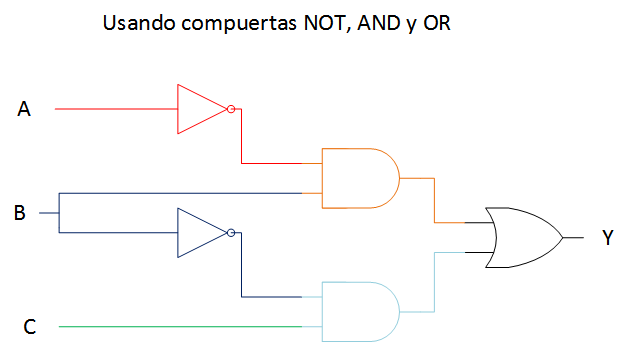
\includegraphics[scale=0.8]{../3-TruthTable/Circuito AND, OR ,NOT.png}
\end{center}
Este circuito hubiese requerido el uso de 3 circuitos integrados. 
Por otro lado, un analisis un poco más profundo permite ver que la realización de dicho circuito en su equivalente en con compuertas \emph{NAND} es menos costoso en terminos monetarios. La razón de esto es que requiere unicamente 2 circuitos integrados

\begin{center}

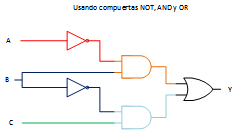
\includegraphics[scale=0.8]{../3-TruthTable/Circuito Logico.png}

\end{center}	